\section{Einführung}
Ein Mol ist eine Stoffmenge von ca. \num{6.022e23} Teilchen, was der Anzahl von Atomen in \SI{12}{g} $\prescript{12}{}{\mathbf{C}}$ entspricht.
Die molare Masse $M$ eines Stoffes ist dann die Masse eines Mols in der Einheit \si{g/\mole} und lässt sich aus einer Probe mit Masse $m$ und Stoffmenge $\nu$ berechnen:
\begin{equation}
	M=\frac{m}{\nu}
\label{eq:molmasse}
\end{equation}

\subsection{Dampfdichtemethode}
Bei der Dampfdichtemethode wird die molare Masse aus der Volumenausdehnung bei bekanntem Druck und Temperatur mithilfe der idealen Gasgleichung
\begin{equation}
	pV=\nu RT
\label{eq:gasgleichung}
\end{equation}
ermittelt.

\begin{figure}[h]
  \centering
  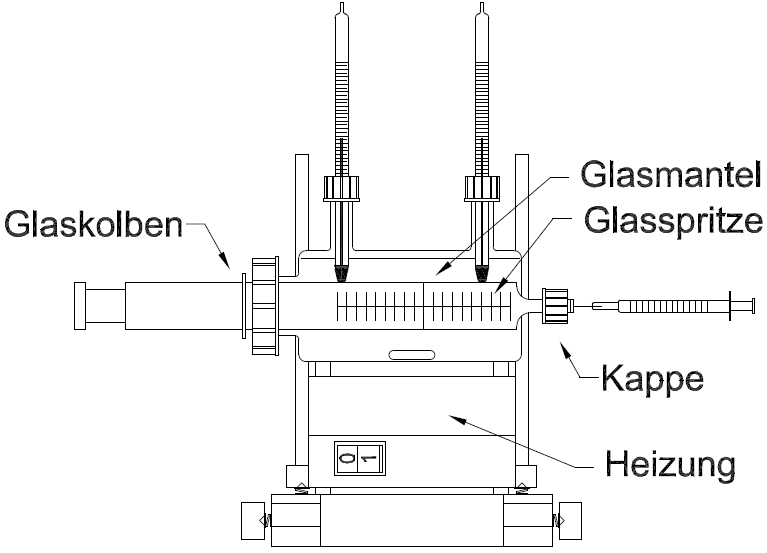
\includegraphics[width=.7\textwidth]{res/dampfdichte}
  \caption{Versuchsaufbau zur Dampfdichtemethode\footcite{anleitung-ss2015}.}
  \label{fig:dampfdichteaufbau}
\end{figure}
Die molare Masse der Probesubstanz lässt sich aus den Werten unter Normalbedingungen für Molvolumen $V_{m0}$, Druck $p_0$ und Temperatur $T_0$, und den im Versuch gemessenen Werten für Druck $p$, Temperatur $T$ und Volumen $V$ berechnen:  

\begin{equation}
	M=m\frac{V_{m0}}{V}\frac{p_0}{p}\frac{T}{T_0}
\label{eq:dampfdichte}
\end{equation}

Beim Wiegen muss der Auftrieb in Luft beachtet werden. Wird eine Spritze einmal leer ($m_1$) und einmal mit einer Flüssigkeit gefüllt ($m_2$) auf derselben  elektrischen Wage gewogen, so kann mit dem Volumen der Flüssigkeit $V_{\text{Fl}}$ und der Dichte von Luft $\rho_L=\SI{1.204}{g/L}$ die vom Auftrieb korrigierte Masse der Flüssigkeit berechnet werden:
\begin{equation}
	m_{\text{Fl}}=(m_2-m_1)+\rho_L V_{\text{Fl}}
\label{eq:auftrieb}
\end{equation}
Da für ein Volumen von $V\leq\SI{0.2}{ml}$ der Korrekturterm kleiner als $\SI{1}{mg}$ ist und die im Praktikum verwendete Waage nur bis auf $\SI{10}{mg}$ genau misst, wird dies im folgenden vernachlässigt.

\subsection{Gefrierpunktserniedrigung}
Wird eine Substanz in einem Lösungsmittel gelöst, so verringert sich der Dampfdruck im Vergleich zum reinen Lösungsmittel um $\Delta p_D$. Nach dem Raoultschen Gesetz ist die relative Dampfdruckerniedrigung nur abhängig von der Teilchenanzahl der Substanz $\nu_S$ bzw. des Lösungsmittels $\nu_L$, aber unabhängig von der Art der Teilchen:
\begin{equation}
	\frac{\Delta p_D}{p_D}=\frac{\nu_S}{\nu_L}
\label{eq:raoult}
\end{equation}
Wie in \cref{fig:gefrierpunkt} zu sehen, sinkt der Gefrierpunkt der Lösung aufgrund des verringerten Dampdruckes um $\Delta T$. Hieraus lässt sich die molare Masse der gelösten Substanz errechnen:
\begin{equation}
	M_S=K\frac{m_S}{m_L}\frac{1}{\Delta T}
\label{eq:gefrier}
\end{equation}
$m_S$ ist die Masse der gelösten Substanz, $m_L$ die Masse des Lösungsmittels und $K$ ist die kryoskopische Konstante, welche vom Lösungsmittel abhängig ist und über die molare Schmelzenthalpie berechnet werden kann.
\begin{figure}[h]
  \centering
  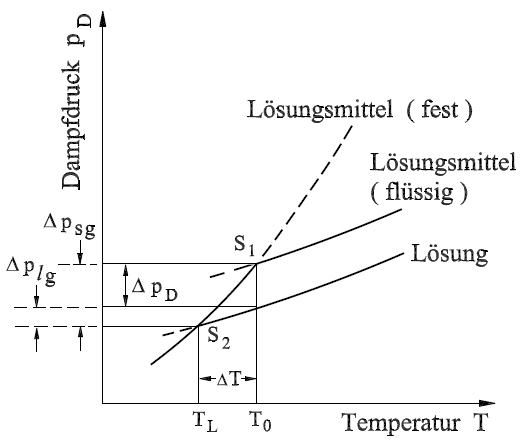
\includegraphics[width=.7\textwidth]{res/gefrierpunkt}
  \caption{Dampfdruckkurven von Lösung, flüssigem und festem Lösungsmittel\footcite{anleitung-ss2015}.}
  \label{fig:gefrierpunkt}
\end{figure}
\null\clearpage\null\clearpage
\refstepcounter{section}
\addcontentsline{toc}{section}{\protect\numberline{\thesection}Versuch}

\refstepcounter{subsection}
\addcontentsline{toc}{subsection}{\protect\numberline{\thesubsection}Bestimmung der molaren Masse einer Probesubstanz durch das
Dampfdichteverfahren}
\refstepcounter{subsubsection}
\addcontentsline{toc}{subsubsection}{\protect\numberline{\thesubsubsection}Ethanol}
\null\clearpage
\refstepcounter{subsubsection}
\addcontentsline{toc}{subsubsection}{\protect\numberline{\thesubsubsection}Cyclohexan}

\refstepcounter{subsection}
\addcontentsline{toc}{subsection}{\protect\numberline{\thesubsection}Bestimmung der molaren Masse einer Probesubstanz durch seine
Gefrierpunktserniedrigung}
\null\clearpage\null\clearpage
\refstepcounter{section}
\addcontentsline{toc}{section}{\protect\numberline{\thesection}Diskussion}

\refstepcounter{subsection}
\addcontentsline{toc}{subsection}{\protect\numberline{\thesubsection}Bestimmung der molaren Masse einer Probesubstanz durch das
Dampfdichteverfahren}

\refstepcounter{subsection}
\addcontentsline{toc}{subsection}{\protect\numberline{\thesubsection}Bestimmung der molaren Masse einer Probesubstanz durch seine
Gefrierpunktserniedrigung}